\documentclass[10pt,a4paper]{report}
\usepackage[latin1]{inputenc}
\usepackage{amsmath}
\usepackage{amsfonts}
\usepackage{amssymb}
\usepackage{graphicx}
\usepackage{hyperref}
\usepackage{multicol}
\usepackage[margin=0.5in]{geometry}
\usepackage{tikz}
\usepackage{romannum}
\usepackage{listings}
\usetikzlibrary{arrows,shapes.gates.logic.US,shapes.gates.logic.IEC,calc}
\usepackage{titlesec}
\titlespacing{\subsection}{1pt}{\parskip}{3pt}
\titlespacing{\subsubsection}{0pt}{\parskip}{-\parskip}
\titlespacing{\paragraph}{0pt}{\parskip}{\parskip}
\newcommand{\myvec}[1]{\ensuremath{\begin{pmatrix}#1\end{pmatrix}}}
\let\vec\mathbf

\begin{document}

\centering {
\includegraphics[scale=0.07]{IIT.png}} \vspace{3mm}\\ \raggedleft Name:Somisetty.Kedareswari\vspace{2mm}\\ \raggedleft Roll No.: FWC22049\vspace{2mm}\\ \raggedright Sep 2022 \hspace{12cm} \raggedleft mail2kedari@gmail.com \vspace{10mm}
\\ \centering \Large \textbf{MATRIX ASSIGNMENT} \normalsize \vspace{15mm}
\begin{multicols}{2}
\section{Problem:}  Let C be the circle with centre (0, 0) and radius 3 units. To find the equation of the locus of the mid points of the chords of the circle C that subtend an angle of 2$\pi$/3 at its \raggedright center\vspace{3mm}
\section{Solution}
The input parameters for this construction are
\begin{center}
\begin{tabular}{|c|c|c|}
  \hline
  \textbf{Symbol}&\textbf{Value}&\textbf{Description}\\
  \hline
  r & 3cm & Radius of a circle given as 8cm\\
  \hline
  $\angle{AOB}$ & $120^0$ & Angle between two chords\\
  \hline 
  O & $\myvec{0\\0}$ & Centre Point\\
  \hline
\end{tabular}
\end{center}
\raggedright\textbf{Caluclating Locus:} \\
 \centering  Let $\theta1=30^0$ and $\theta2=120^0-\theta1 $
 \vspace{5mm}
 \\ Chord A=$\myvec{rcos \theta1 \\ rsin \theta1 }$ \\
 \vspace{5mm}
 Chord B=$\myvec{rcos \theta2 \\ -rsin \theta2 }$ \\
 \raggedright Upon Simplification we get \\ 
   \centering   A=$\myvec{2.59 \\ 1.5}$ and  B=$\myvec{0 \\ -3 }$ \\ 
    \vspace{5mm}
\raggedright Finding Mid-Point
      \begin{equation} M=(A+B)/2. \end{equation} \\
    \raggedright Upon Simplification we get \\ 
       \centering M=$\myvec{1.299\\ -0.75 }$ \\
\raggedright Finding Radius of locus(circle)
 \begin{equation} r2 \implies (O-M)=\sqrt{M.M^T} 
 \end{equation}\\ 
 \centering $r2=\frac{9}{4}$ \\
 \raggedright Finding Circle Equation
   \\
   \begin{equation} 
     (x-x0)^2+(y-y0)^2=r2^2
   \end{equation}\\ 
   \begin{equation} 
   Where, (x0,y0)=\myvec{0\\0} 
  \end{equation} \\
 \raggedright Upon Simplification we get \\
   \centering $x^2+y^2= r2^2$ \\
 \raggedright Equation of locus is
   \begin{equation}
    x^2+y^2= \frac{9}{4}
   \end{equation}
   
 \begin{center}
Below python code realizes the above construction : 
\fbox{\parbox{8.5cm}{\url{https://github.com/kedareswari200/fwc-moudle1/blob/Matrix_Circle/cir.py}}}
\end{center}
 \section{Construction}
   \begin{center}
  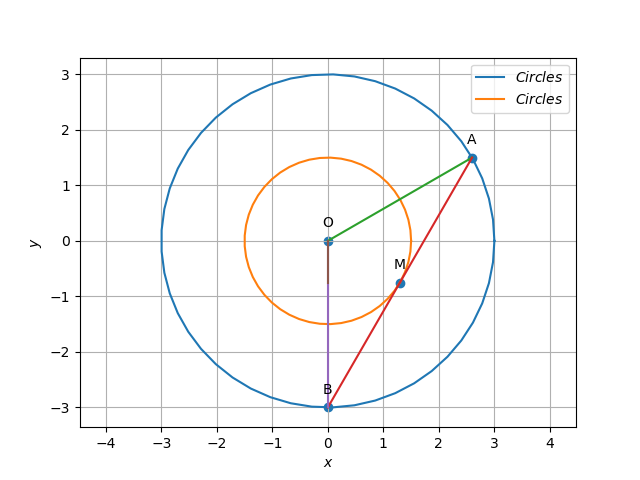
\includegraphics[scale=0.5]{Fig.png}
    \end{center}
\vspace{3cm}
\end{multicols}

\end{document}